\documentclass{article}
 \usepackage[table,xcdraw]{xcolor}
%\documentclass[twocolumn,showpacs,showkeys,preprintnumbers,amsmath,amssymb]{revtex4}
\usepackage[american]{babel}
\usepackage[latin1]{inputenc}
\usepackage{graphicx}
\usepackage[colorinlistoftodos]{todonotes}
\usepackage{booktabs}
 \usepackage{booktabs}
\usepackage{float}
\usepackage{subcaption}
\usepackage{indentfirst}
\usepackage{natbib} 
\begin{document}


\title{Some title}

%\vspace{1cm}

\author{Marcelo V. Maciel \and Andr\'e C. R. Martins\\
	%}
	%\email{amartins@usp.br}
	%\affiliation{%
	NISC - EACH, Universidade de S\~ao Paulo\\
	Av. Arlindo B\'etio, 1000, S\~ao Paulo, 03828-080, Brazil}

%\author{Andr\'e C. R. Martins\\
	%}
 %\email{amartins@usp.br}
 %\affiliation{%
%NISC - EACH, Universidade de S\~ao Paulo\\
%Av. Arlindo B\'etio, 1000, S\~ao Paulo, 03828-080, Brazil}
 

\date{}


\maketitle
%\vspace{0.3cm}

%\center{\Large\bf Segundo autor}
%\center{\large\bf Afilia��o}


\begin{abstract}
	
	
	%\keywords{}
	%\pacs{}
\end{abstract}


\section{Introduction}

 % Incluir aqui a parte sobre teoria pol�tica, um par�grafo � suficiente, a princ�pio.

In this paper, we will propose a opinion dynamics model
\cite{castellanoetal07,galam12a,galametal82,galammoscovici91,sznajd00,deffuantetal00,martins08a}
to explore the consequences of the existence of issues that can be interpreted
as opinions over an one-dimensional axis. It's usual to think
  about policy alternatives and agents' preferences spatially (geometrically),
  that is, through a mapping from similarity to proximity
  \cite{downs1957economic, laver2014measuring}. The model then captures the
  daily notion of parties or policies being more ``to the left'' or ``right''
  than others, that is, if they're similar then they're closer
  \cite{van2005political, miller2015spatial}. Major opinions, including
political ones, tend to be formed from how each person feels about a number of
issues. Locating someone in a left versus right or liberal versus conservative
axis, \textcolor{blue}{ therefore}, requires inspecting the opinions of that
person in not only one but a number of different issues that constitute the
ideological positioning \cite{benoit2006party}.

While it would make sense to consider different issues as having components in
more than one single dimension \cite{vicenteetal08b}, looking at the problem as
one-dimensional can be justified in several ways. We can certainly see this as a
first approximation along the most relevant dimension. In this case, we are
simply investigating the projection of higher-dimensional problems along a
direction where variation seems especially important. And, from the point of
view of applications, it is usual to find discussions to be simplified over a
main disagreement.  Even though there are many variants of this
  modeling strategy, for our work what matters is that this naturally leads to
  the use of continuous opinion models such as the Bounded Confidence (BC)
models \cite{deffuantetal00,hegselmannkrause02}. While discrete models
\cite{galametal82,galammoscovici91,sznajd00} can be very useful at describing
choices, they are not easiest way to represent strength of opinion. Discrete
models also do not naturally provide a scale where we can compare opinions and
decide which one is more to the right or more liberal.

On the other hand, continuous models are not particularly well suited for
problems involving discrete decisions. As we will not deal with those kinds of
problems here, they are a natural choice. Indeed, continuous opinions models
have been proposed for several different problems on how opinions spread on a
society \cite{deffuantetal02a,weisbuchetal05}, from questions about the spread
of extremism
\cite{amblarddeffuant04,gargiulomazzoni08a,franksetal08a,alizadeh14a,Albi2016,Mai2017}
to other issues such as how different networks
\cite{Kurmyshev2011,Acemoglu2011,Das2014,Hu2017} or the uncertainty of each
agent \cite{deffuant06} might change how agents influence each other.

Here, we will use a continuous opinion model created by Bayesian-like reasoning
\cite{martins08c}, inspired by the Continuous Opinions and Discrete Actions
(CODA) model \cite{martins08a,martins12b}. The model was shown previously
\cite{martins08c} to provide the same qualitative results as BC models. While a
little less simple, the Bayesian basis make for a more clear interpretation of
the meaning of the variables, as we extend the model and need to interpret the
new results, and is consistent with a boundedly rational
  variant interpretation of the spatial model of political decision making
  \cite{humphreys2010spatial,ostrom1998behavioral}.

We will also study variations of our model where the function of trust $p^*$
will not be influenced by the distance between the opinions of the agent and the
neighbor on the specific issue they are debating. Instead, we will test two
other cases: in the first alternative, \(p^*\) will be determined by the
distance between the neighbor and the agent average opinions (the \(p^{**}\)
case); in the second alternative, \(p^*\) is derived from the opinion of the
neighbor and the average opinion of the agent ( the \(p^{***}\) case). The idea
here is to make the behavior of our agents closer to what experiments show about
human reasoning. We have observed that our reasoning about political problems
can be better described as ideologically motivated
\cite{jostetal03a,taberlodge06a,Claassen2015a}. Indeed, our opinions tend to
come in blocks even when the issues are logically independent \cite{jervis76a}.
Our reasoning abilities seem to exist more to defend our main point of views
\cite{mercier11a,merciersperber11a} and our cultural identity \cite{kahanetal11}
than to find the best answer. In that context, evaluating other by how they
differ from us as a whole, instead of in each issue, is a model variation worth
exploring.
 
\section{The Model}


  The model is an agent-based social simulation \cite{de2014agent}. At the initial
condition of the simulation we have a population of \(N\) agents which have an
ideological profile
\(I_i
=
(
(o_{i, 1}, \sigma),
\ldots,
(o_{i, n}, \sigma)
)
\)
, where \(n\) is the number of issues, \(o\) is
the opinion about the issue and \(\sigma\) is a global
variable which can be interpreted as the uncertainty about the issue
\cite{martins12b}. Another attribute is the agent's ideological position at the
dimension of interest, or ideal point \cite{armstrong2014analyzing}, which we
treat as the arithmetic mean of its opinions in each issue
\(
x_i
=
\frac{1}{n}
\sum_{k=1}^{n}
o_{k}
\).


The initial \(o_i\)s for each issue are sampled from Beta\((\alpha, \beta)\)
distributions where each agent is associated with its own pair
\( (
\alpha
\in [1.1, 100],
\beta
\in [1.1, 100]
)
\)
.
The reason for this is that if we sample the \(o\)s from an Uniform distribution
as we increase the number of issues (\(n\)) the closer to the center of the
dimension the agents' ideological position (\(x\)) would be.
\todo[color=yellow!40]{maybe refactor this sentence?} Using a Beta distribution
prevents this, lets the initial \(o\)s of each agent to be correlated, since
they're drawn from the agent's own Beta, and lets us have an initial population
of agents with ideological positions distributed along the dimension, instead of
clustered around the center.


For its part, \(\sigma\) is a global variable, that is, a parameter of the
model. A certain proportion of the agents will have an unique \(\sigma_{i,k} =
1e-20\), so that we can control for the impact of \textit{intransigent} agents
on the model dynamics \cite{deffuant2002can}. How many agents are intransigent
is also a parameter (coded as \textit{p$\_$intran} ), and such \(\sigma\) is
established at the initial condition by sampling the issue index from the
\(I_i\)'s length.

An iteration of the simulation is the application of two
  procedures: the opinion update through social influence and a random opinion
  update (noise). In the social influence procedure we draw a single agent \(i\)
  from the population. We then draw another agent \(j\) from the population.
  Afterwards, we draw one of the issues \(k \in (1 , \ldots, n)\) so that we
  have the corresponding pairs (\(o_{i,k}, o_{j,k}\)) and (\(\sigma_{i,k},
  \sigma_{j,k}\)). Finally, the agent \(i\) updates its opinion (\(o_{i,k}\))
  following the equation
  \[
    o_{i,k}(t+1) =
    p^{*}
    \frac{o_{i,k}(t) + o_{j,k}(t) }{2}
    +
    (1 - p^{*})
    o_{i,k}(t).
  \]

  Wherein 
  \[
   p^{*}
    =
  \frac{
      p \frac{1}{\sqrt{2 \pi} \sigma_i}
      e^{- \frac{ (\Delta_{ij})^2}{2 \sigma_i^2}}
    }{
      p
      \frac{1}{\sqrt{2 \pi} \sigma_i}
    e^{- \frac{ ( \Delta_{ij})^2}{2 \sigma_i^2}}
    +
    (1 - p)
  }.
\]


The \(\Delta_{ij} \) term is equal to \( o_{i,k} (t) - o_{j,k} (t)\). As
mentioned, we also test cases in which it's equal to \( x_i(t) - x_j(t) \) ( the
\(p^{**}\) case ) and to \(x_{i}(t) - o_{j,k}(t)\) ( the \(p^{***}\)). \(p\),
for its part, is a global parameter used to model the likelihood of the other
agent's (\(j\)) opinion being true \cite{martins12b}.

Furthermore, there is the noise: we draw another agent \(i\) whose opinion \(
o_{i,k}(t+1)\) is equal to \(o_{i,k}(t) + r\) where \(r\) is taken from a Normal
distribution of mean 0 and standard deviation \(\rho\). \(\rho\) is then a
global parameter of the simulation. From a theoretical point of view the noise
is justified as a way of accounting for the effect of factors not related to
social influence that make the agents change their opinion about issues
\cite{flache2017}. A further methodological justification is that small
perturbations in the local behavior of agents may lead to drastic changes in
systemic properties \cite{macy2015signal}. If an agent \(i\) is intransigent in
an issue \(k\) it won't randomly change its \(o_{i,k}\) opinion if its chosen by
the noise algorithm. Moreover, if \(o_{i,k}(t) + r > 1\) then \( o_{i,k}(t+1) =
1\). Likewise, if \(o_{i,k}(t) + r < 0 \) then \( o_{i,k}(t+1) = 0\).

  \section{Model Results}

  \todo[inline,color=yellow!2]{i'm gonna create the structure and then polish}
  To have a general understanding about the model behavior we first established
  the bounds of the parameters:

% Please add the following required packages to your document preamble:
% \usepackage{booktabs}
% \usepackage[table,xcdraw]{xcolor}
% If you use beamer only pass "xcolor=table" option, i.e. \documentclass[xcolor=table]{beamer}
% Please add the following required packages to your document preamble:
% \usepackage{booktabs}
% \usepackage[table,xcdraw]{xcolor}
% If you use beamer only pass "xcolor=table" option, i.e. \documentclass[xcolor=table]{beamer}
  \begin{table}[H]
    \centering
\begin{tabular}{@{}|l|l|l|l|l|l|@{}}
\toprule
\rowcolor[HTML]{EFEFEF} 
$\sigma$ & $n$ & $p$ & $p\_intran$ & $N$ & $\rho$ \\ \midrule
$[0.01, 0.5]$ & $[1, 10]$  & $[0.1, 0.99]$ & $[0.0, 0.1]$ & $[500, 5000]$ & $(0.0, 0.1]$ \\ \bottomrule
\end{tabular}
\caption{Parameters' Bounds}
\end{table}

To sweep the parameter space we sample 70.000 parameterizations taken from
quasi-random low-discrepancy sequences \cite{saltelli2008global}, that generate
evenly spaced points. After running the simulation for 1.000.000 iterations we
take the  standard deviation of the population mean opinions (\(Ystd\)) as
a system final state measure. Histograms of the initial condition viz-a-viz
the three cases (\(p^{*}, p^{**}, p^{***}\)) final state lets us understand the
general tendency impinged by the update rules:

\begin{figure}[H]
  \centering
  \caption{foo}
    \begin{subfigure}[b]{0.49\textwidth}
      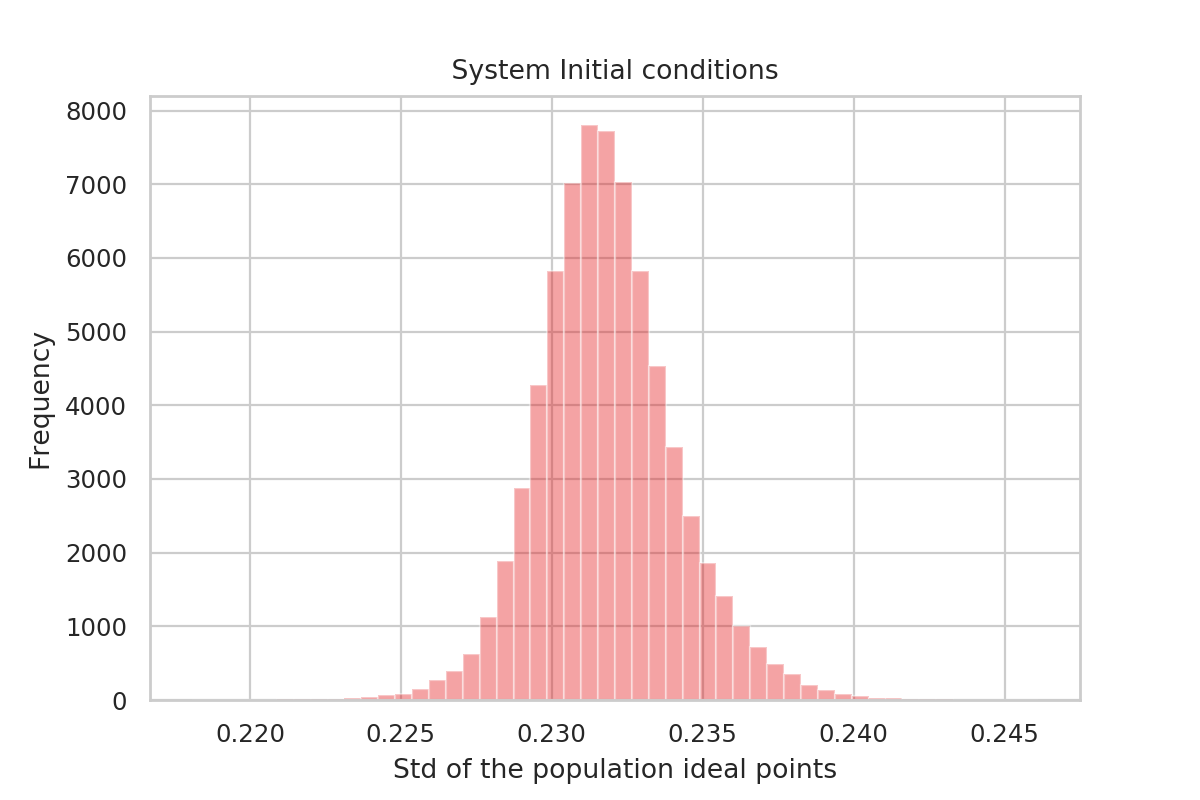
\includegraphics[width=\textwidth]{img/initstd.png}
%      \caption{\( n\_issues = 1,  \sigma = 0.1\) }
    \end{subfigure}
    \begin{subfigure}[b]{0.49\textwidth}
      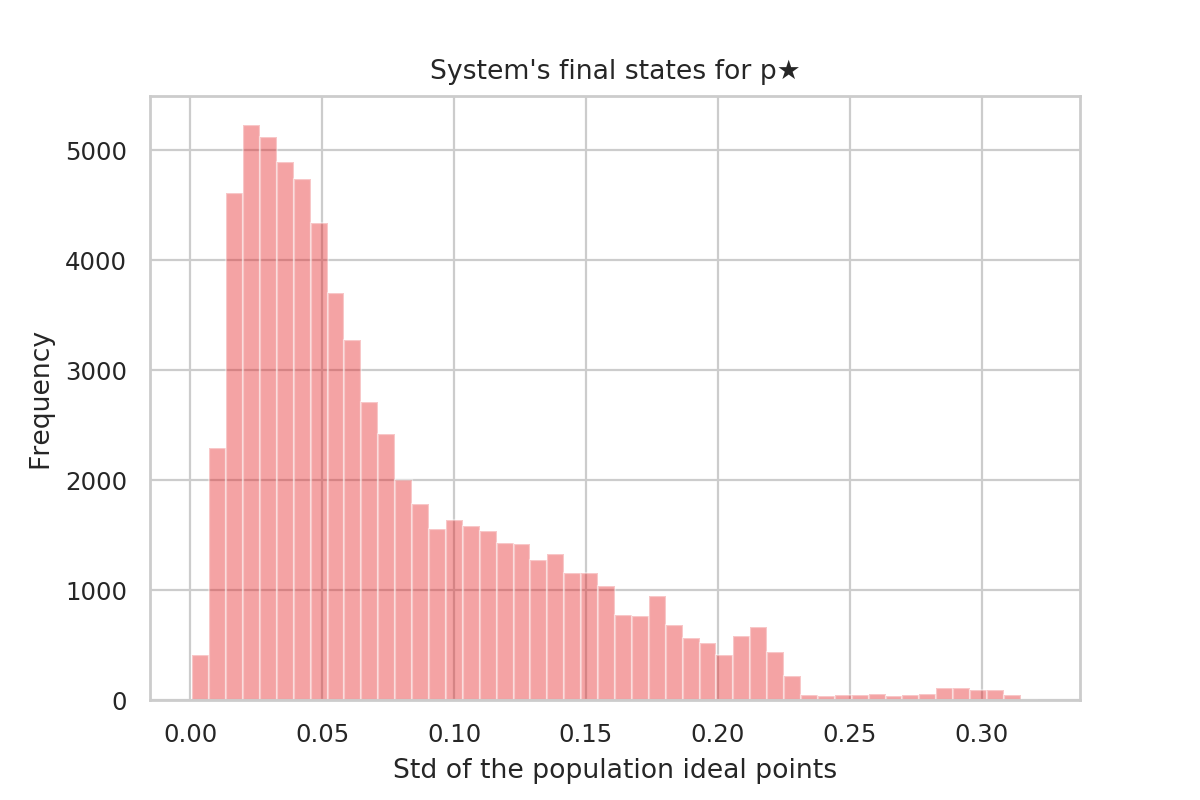
\includegraphics[width=\textwidth]{img/Ystd*.png}
 %      \caption{\(n\_issues = 1, \sigma = 0.02\) }
     \end{subfigure}

     \begin{subfigure}[b]{0.49\textwidth}
       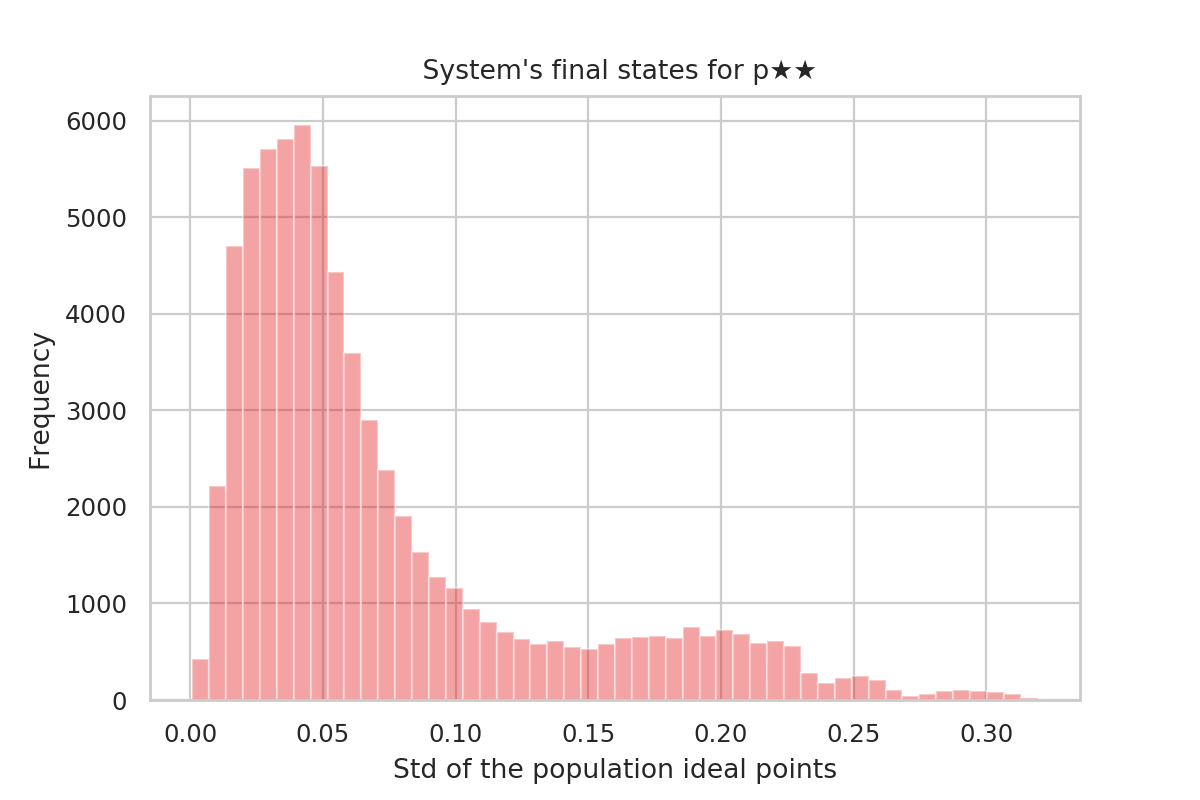
\includegraphics[width=\textwidth]{img/Ystd**.png}
  %     \caption{\(n\_issues = 7, \sigma = 0.1\)}
     \end{subfigure}
     \begin{subfigure}[b]{0.49\textwidth}
       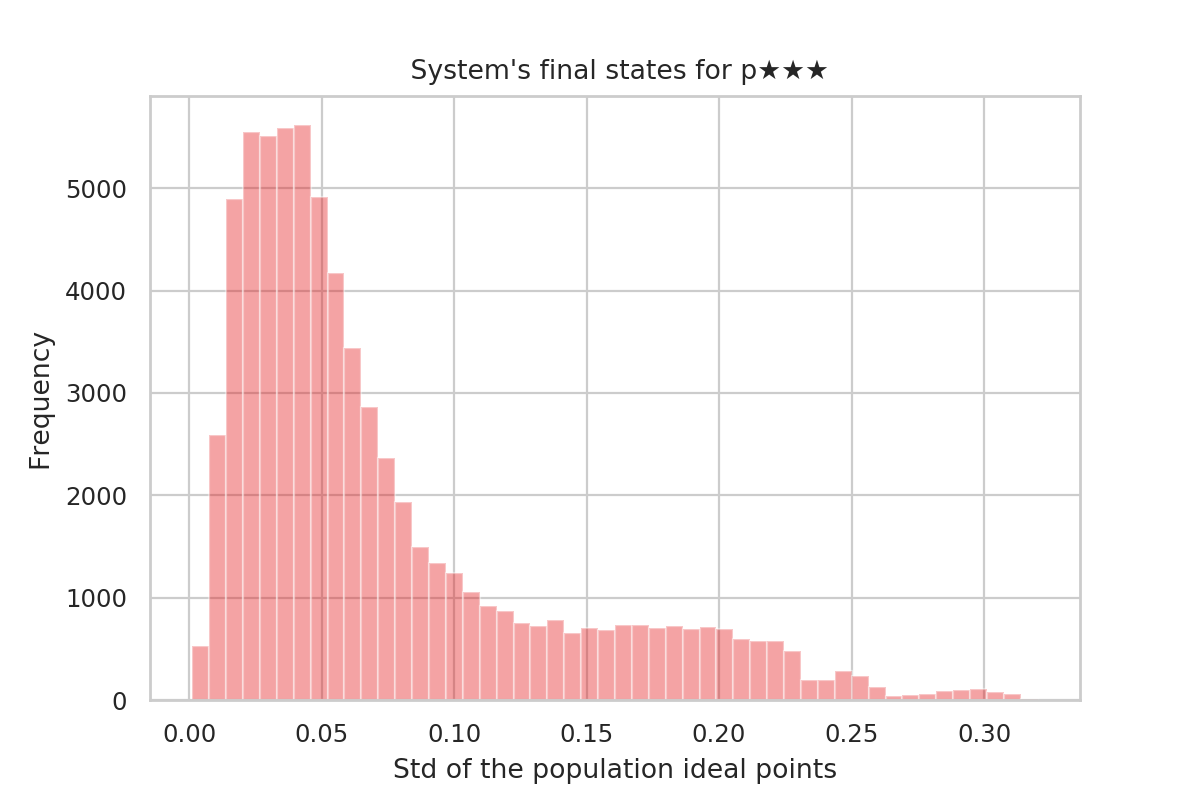
\includegraphics[width=\textwidth]{img/Ystd***.png}
   %    \caption{\(n\_issues = 7, \sigma = 0.02\)}
     \end{subfigure}
      \label{fig:hists}
    \end{figure}

    The general tendency of the model is one of biased assimilation
    \cite{flache2017}. The histograms, however, don't show which parameter is
    the most important to explain this trend. With that in mind we perform a
    Sobol sensitivity analysis \cite{saltelli2000sensitivity} which generate the
    following indexes:

    \begin{figure}[H]
  \centering
  \caption{bar}
    \begin{subfigure}[b]{0.45\textwidth}
      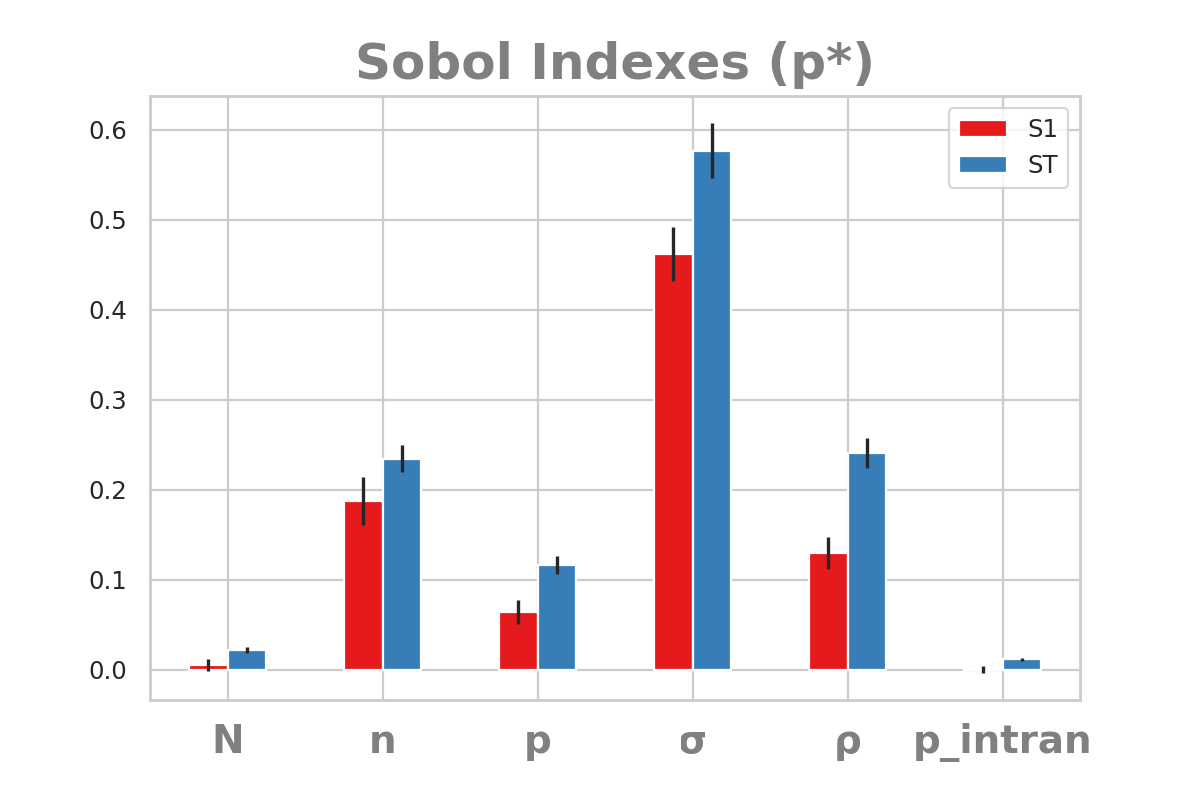
\includegraphics[width=\textwidth]{img/sobolpstar1.png}
%      \caption{\( n\_issues = 1,  \sigma = 0.1\) }
    \end{subfigure}
    \begin{subfigure}[b]{0.45\textwidth}
      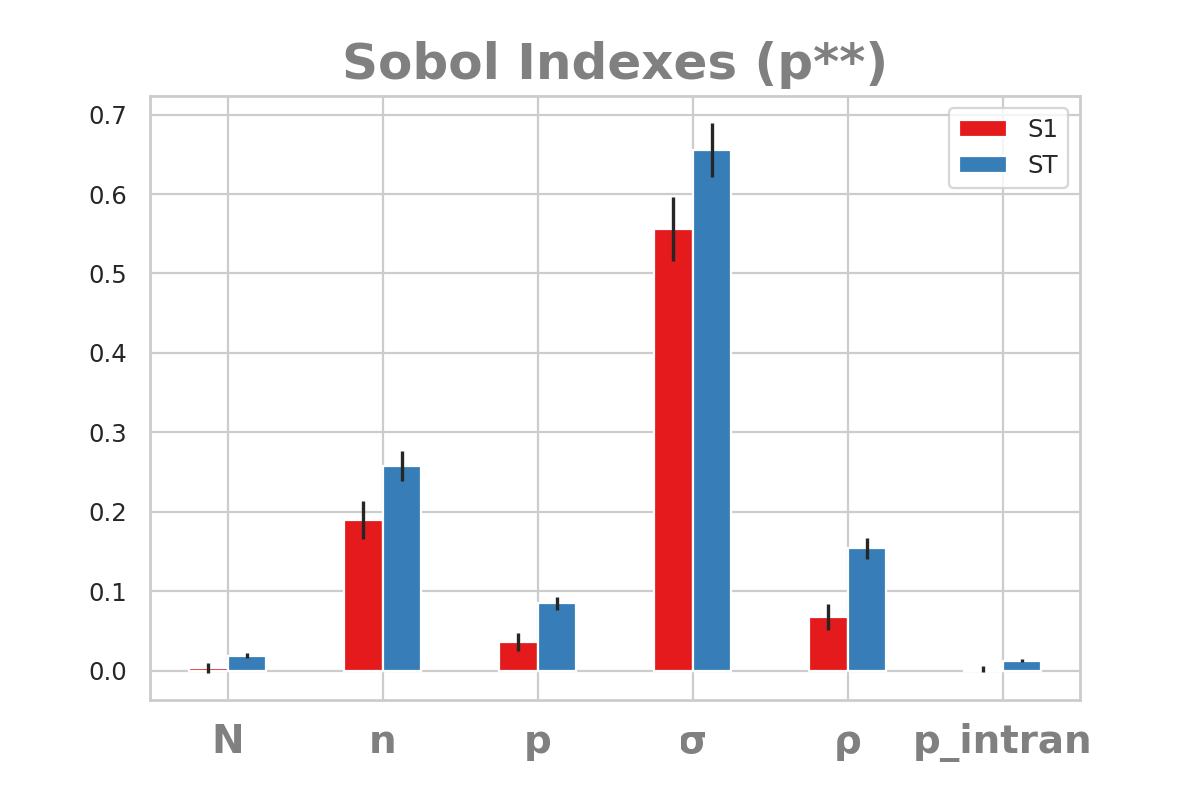
\includegraphics[width=\textwidth]{img/sobolpstar2.png}
 %      \caption{\(n\_issues = 1, \sigma = 0.02\) }
     \end{subfigure}
     \begin{subfigure}[b]{0.5\textwidth}
       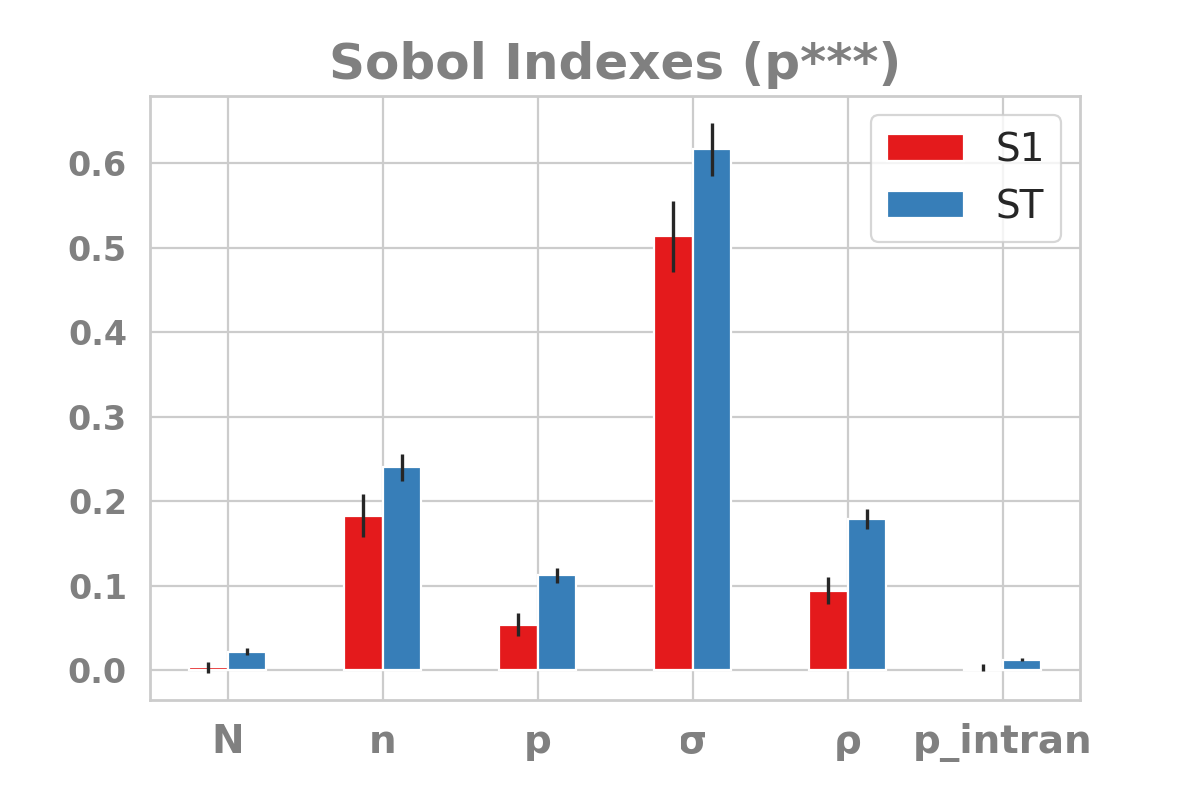
\includegraphics[width=\textwidth]{img/sobolpstar3.png}
  %     \caption{\(n\_issues = 7, \sigma = 0.1\)}
     \end{subfigure}
      \label{fig:sobolstuff}
    \end{figure}

    The sensitivity analysis shows that the most important parameters are :
    \(\sigma, n, \rho\), and that the three cases have the same qualitative
    behavior. \(\sigma\) being the parameter that explains the most the variance
    of the system measure is consistent with \citep{martins12b}, while the
    relevance of the number of issues and the noise is a new result. The
    sensitivity analysis, however, does not show the direction of the impact,
    which we investigate through scatter plots:

        \begin{figure}[H]
  \centering
  \caption{foobar}
    \begin{subfigure}[b]{0.45\textwidth}
      \includegraphics[width=\textwidth]{img/regressionYstd*n_issues.png}
      \caption{\textcolor{red}{'ill fix thix}}
    \end{subfigure}
    \begin{subfigure}[b]{0.45\textwidth}
      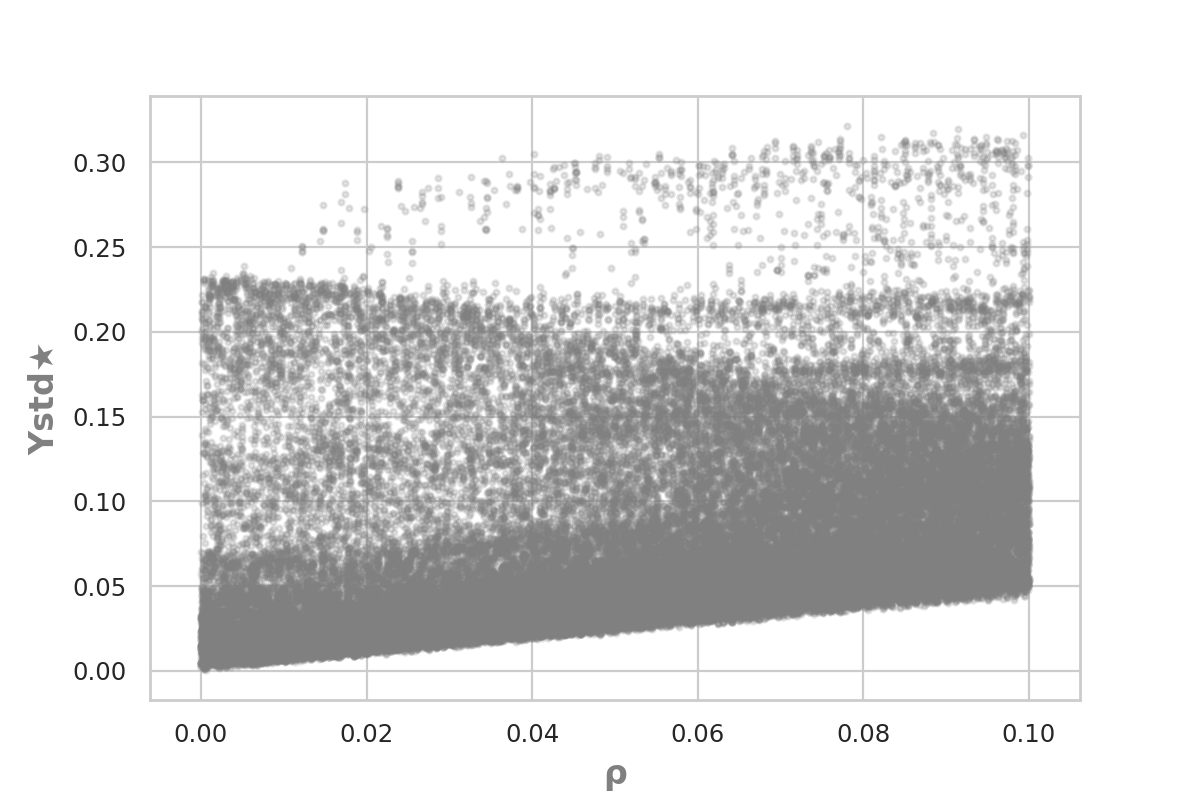
\includegraphics[width=\textwidth]{img/regressionYstd*rho.png}
 %      \caption{\(n\_issues = 1, \sigma = 0.02\) }
     \end{subfigure}
     \begin{subfigure}[b]{0.5\textwidth}
       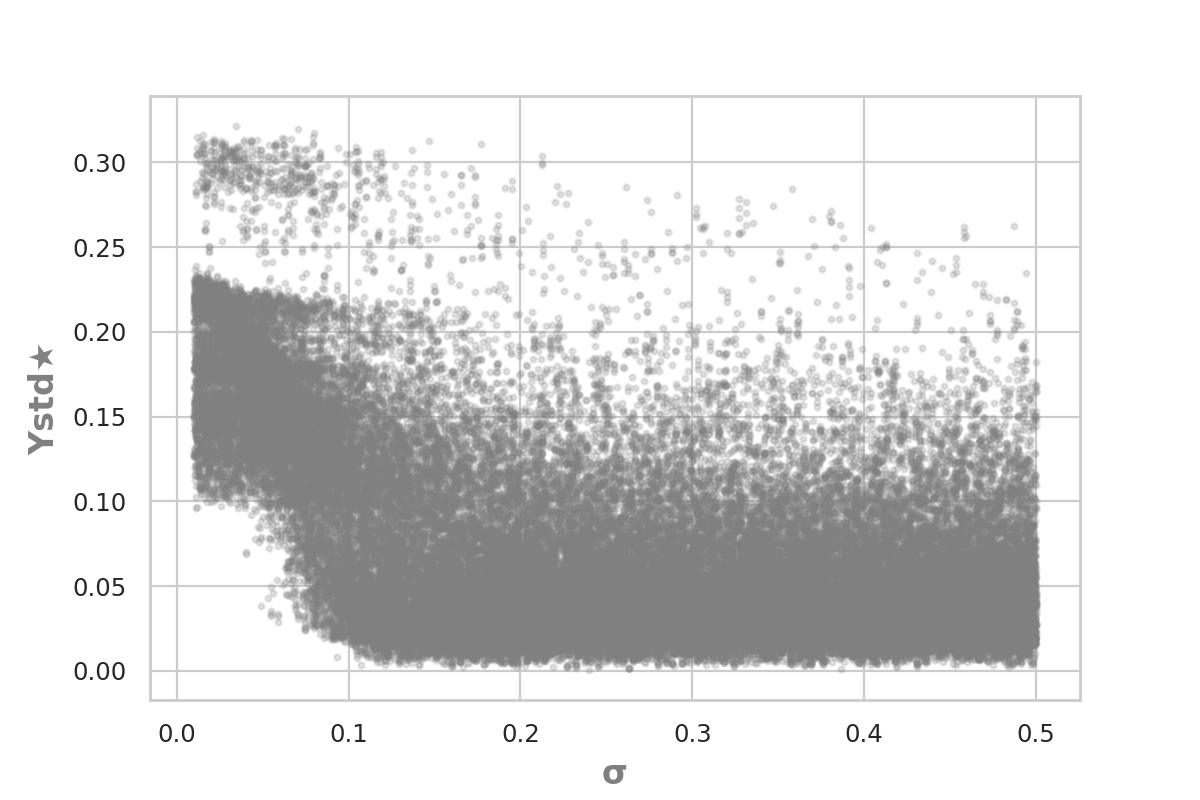
\includegraphics[width=\textwidth]{img/regressionYstd*sigma.png}
  %     \caption{\(n\_issues = 7, \sigma = 0.1\)}
     \end{subfigure}
      \label{fig:scatters}
    \end{figure}

    \todo[inline,color = yellow!20]{the direction will be written} The plots
    show that \(\sigma\) has the same impact on the system whenever its bigger
    than approximately 0.1 Therefore we restrict our following analysis to the
    \((0.0, 0.1 ] \) range. The same can be inferred from \(n> 5\). And the
    effect of \(\rho\) is the expected: the bigger the noise more dispersed is
    the final state of the system.

    After a general investigation we turn to the analysis of specific
    parametizations. For that let's start by fixing the following parameters as
    constants: \(\rho = 0.05 \) ; \(N = 500\) ; \(p\_intran = 0.0\), run the
    simulation for 500.000 iterations, and test combinations of $\sigma = (0.02,
    0.04, 0.1)$ and $ n = (1,5)$. As show by \ref{fig:tseries1}, \(\sigma\) has
    the effect of leading the dynamics of the simulation to the center as it
    increases: the bigger the \(\sigma\) the closest to the mean the population
    is . However,when the number of issues also increases that tendency is not
    clear, since the noise disperses them, even though \(\sigma\) has a bigger
    impact:


        \begin{figure}[H]
  \centering
  \caption{foobarbar}
    \begin{subfigure}[b]{0.45\textwidth}
      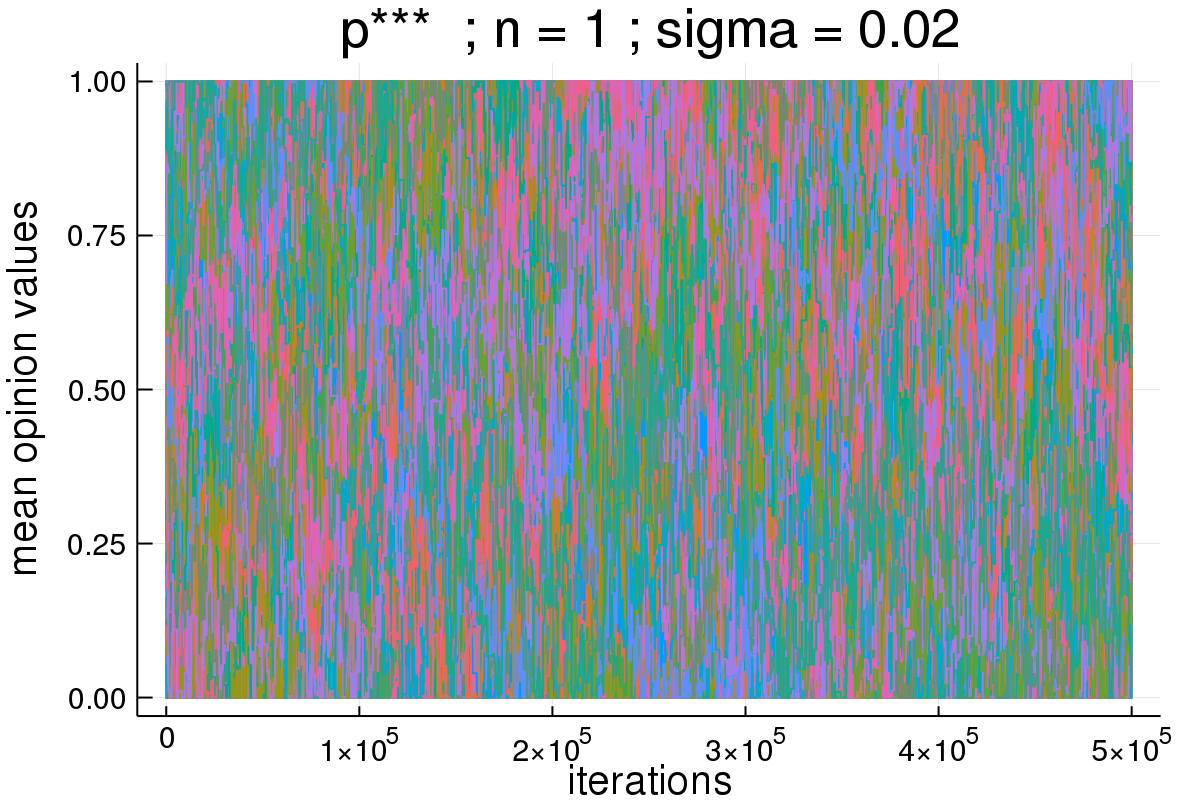
\includegraphics[width=\textwidth]{img/compare-ps/Poodlcalculatep***n1-rho005-sigma002-00intrans.png}
      %\caption{\textcolor{red}{'ill fix thix}}
    \end{subfigure}
    \begin{subfigure}[b]{0.45\textwidth}
      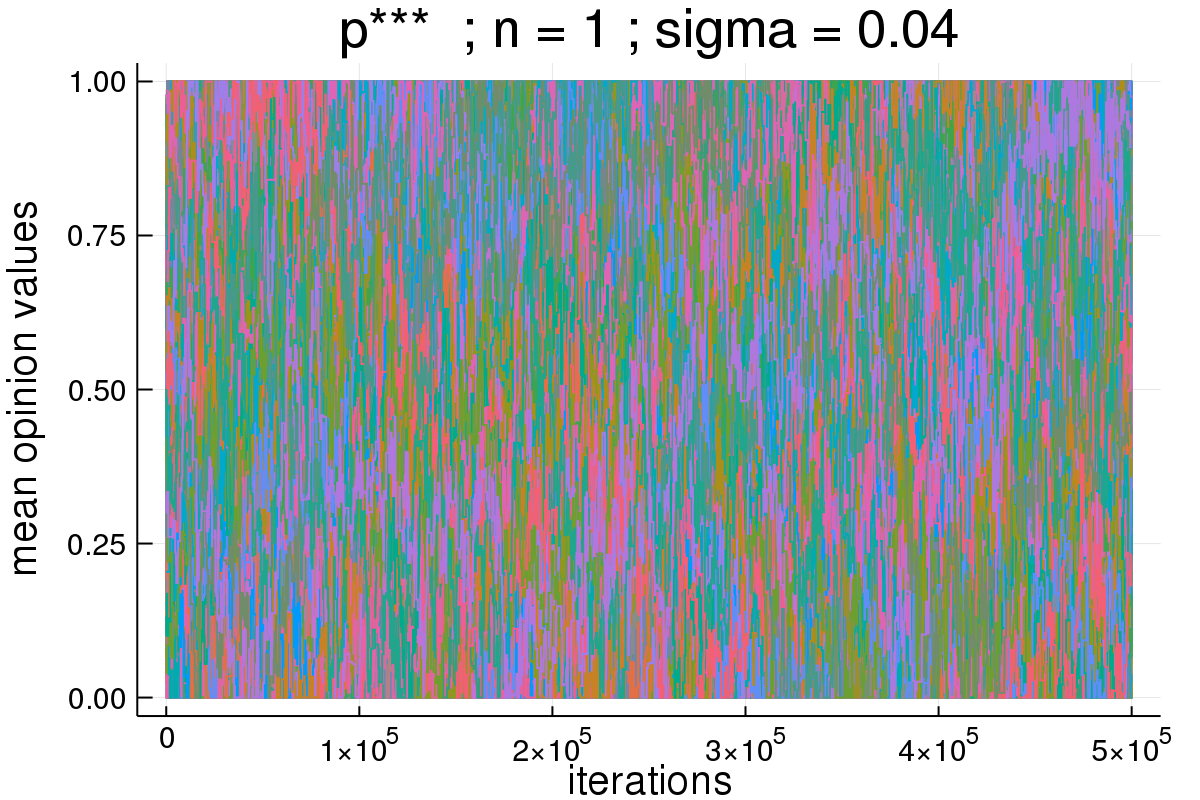
\includegraphics[width=\textwidth]{img/compare-ps/Poodlcalculatep***n1-rho005-sigma004-00intrans.png}
 %      \caption{\(n\_issues = 1, \sigma = 0.02\) }
     \end{subfigure}
     \begin{subfigure}[b]{0.5\textwidth}
       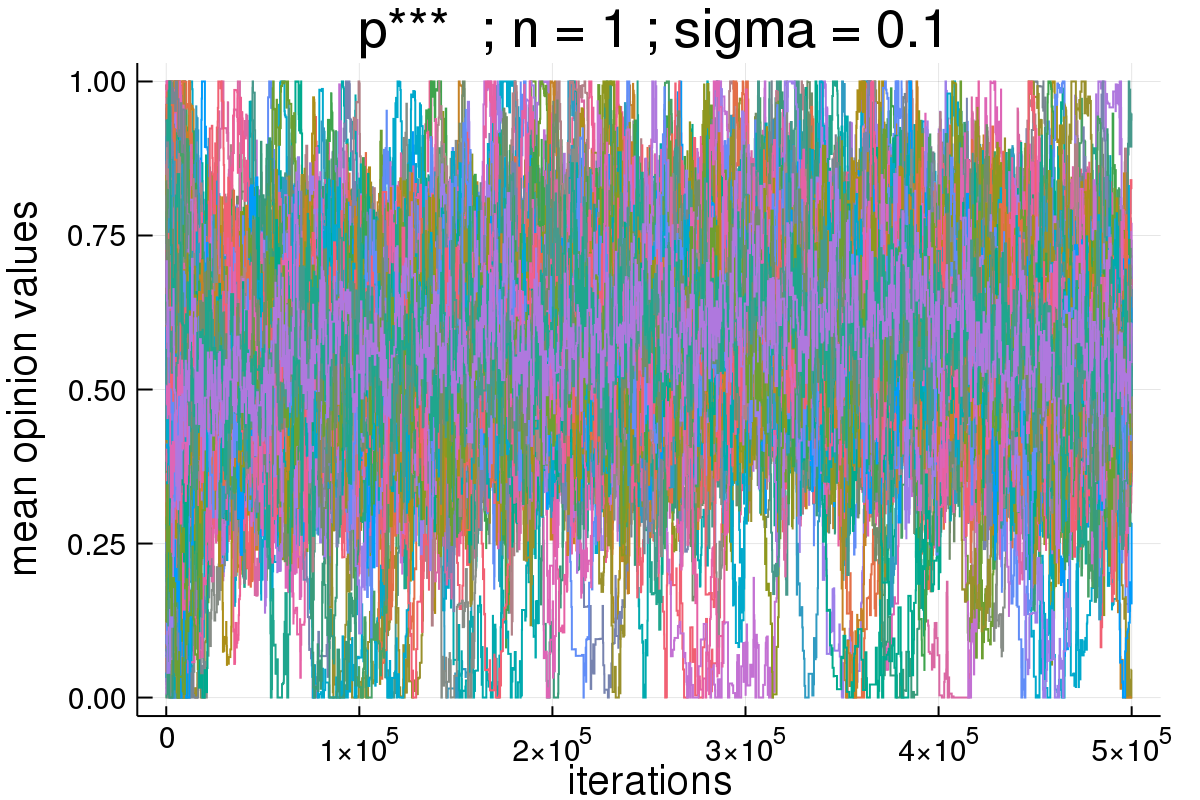
\includegraphics[width=\textwidth]{img/compare-ps/Poodlcalculatep***n1-rho005-sigma01-00intrans.png}
  %     \caption{\(n\_issues = 7, \sigma = 0.1\)}
     \end{subfigure}
      \label{fig:tseries1}
    \end{figure}

    On the other hand, when we also increase the number of issues the
    centralizing effect of \(\sigma \) becomes stronger:

    \begin{figure}[H]
      \centering
      \caption{foofoobarbar}
      \begin{subfigure}[b]{0.45\textwidth}
        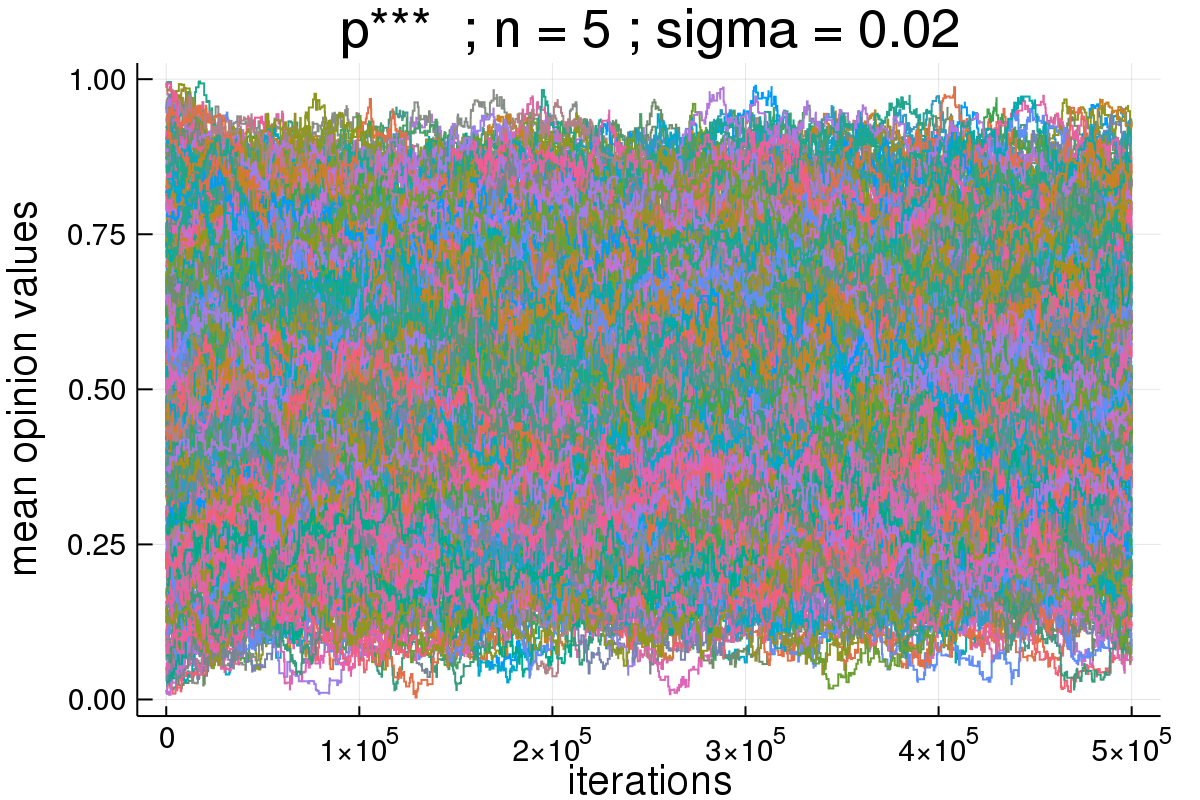
\includegraphics[width=\textwidth]{img/compare-ps/Poodlcalculatep***n5-rho005-sigma002-00intrans.png}
        % \caption{\textcolor{red}{'ill fix thix}}
      \end{subfigure}
      \begin{subfigure}[b]{0.45\textwidth}
        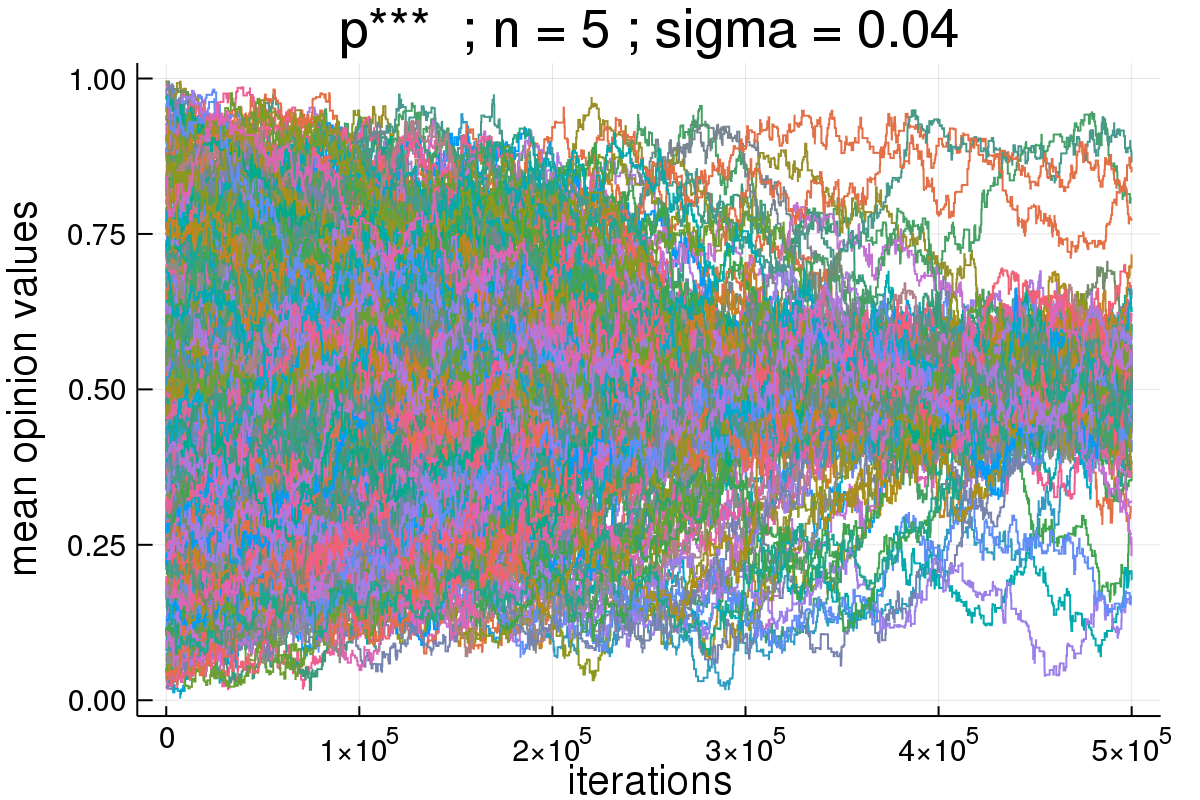
\includegraphics[width=\textwidth]{img/compare-ps/Poodlcalculatep***n5-rho005-sigma004-00intrans.png}
        % \caption{\(n\_issues = 1, \sigma = 0.02\) }
      \end{subfigure}
      \begin{subfigure}[b]{0.5\textwidth}
        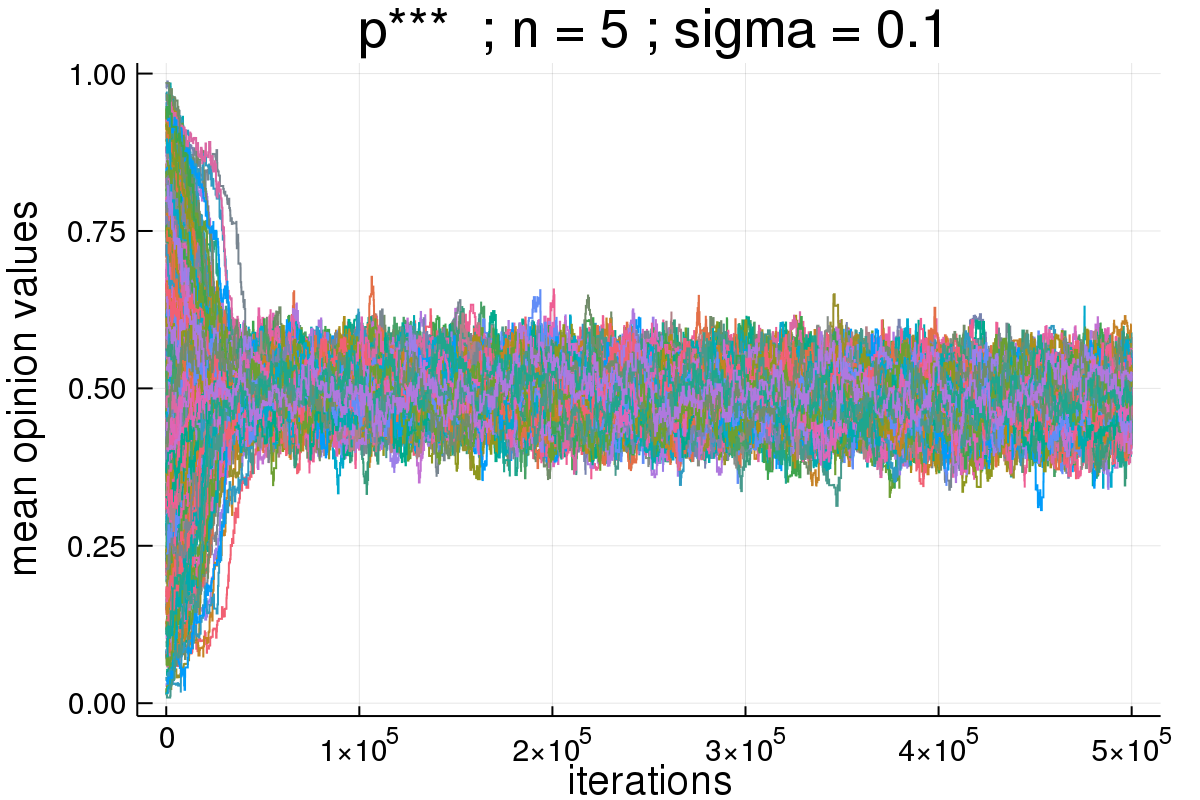
\includegraphics[width=\textwidth]{img/compare-ps/Poodlcalculatep***n5-rho005-sigma01-00intrans.png}
        % \caption{\(n\_issues = 7, \sigma = 0.1\)}
      \end{subfigure}
      \label{fig:tseries2}
    \end{figure}

    The reason for that is : we're measuring the mean opinion values (\(x_i\))
    and \(\rho\) changes a single \(o_i\) at each iteration which means that a
    higher \(n\) implies a lesser impact of \(\rho\) on the mean opinion of the
    agent, since she will have \(n-1\) other opinions stabilizing her mean
    opinion at a point in the opinion spectrum. As \(\sigma\) is the parameter
    that dominates the model update rule it interacts with \(n\), which enforces
    \(\sigma\) effect whenever we test higher \(n\)s. This effect holds even
    when we raise \(\rho\) together with \(n\). Let's use the same
    parameterization as the last plot but with a new \(\rho\) such that \(\rho_2
    = \sqrt{n} * \rho_1 = \sqrt{10} * 0.05\). The interaction between \(n\) and
    \(\sigma\) still happens, with bigger \(n\) stabilizing the noise effect and
    contributing to the centralizing effect of \(\sigma\), even though a bigger
    \(\rho\) leads to a bigger spectrum ``walking''. (\textcolor{red}{refactor
      this paragraph, specially this last sentence}).

    \begin{figure}[H]
      \centering
      \caption{fuba}
      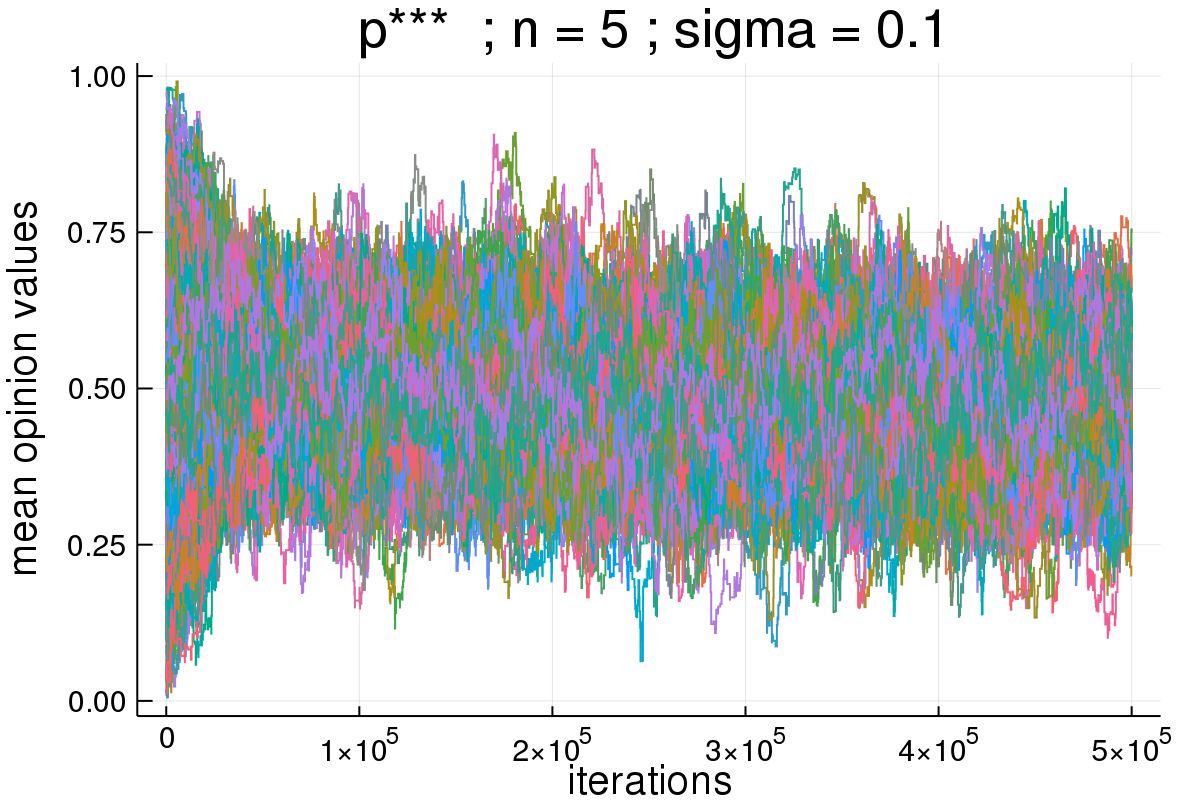
\includegraphics[width=0.9\textwidth]{img/compare-ps/Poodlcalculatep***n5-rho01118033988749895-sigma01-00intrans.png}
      \label{fig:tseries3}
    \end{figure}


    Heretofore we've tested parameterizations with noise, but what happens if we
    lower it to a close to zero value, such as 1e-5? The first difference is
    that the population mean opinion values converge to certain values. In
    parameter combinations in which \(\sigma = 0.1\) the tendency is convergence
    to values close to 0.5. An interesting distinction between the cases in this
    parameterization is that \(p^{**}\) and \(p^{***}\) always converge to 0.5,
    independently of the number of issues. Alternatively, in the \(p^{*}\) case
    this happens when \(n=1\), but when we have \(n=5\) or \(10\) there are
    other values of convergence, more as we increase \(n\), even though the
    centralizing tendency remains
    \begin{figure}[H]
      \centering
      \caption{foofoobarbar}
      \begin{subfigure}[b]{0.45\textwidth}
        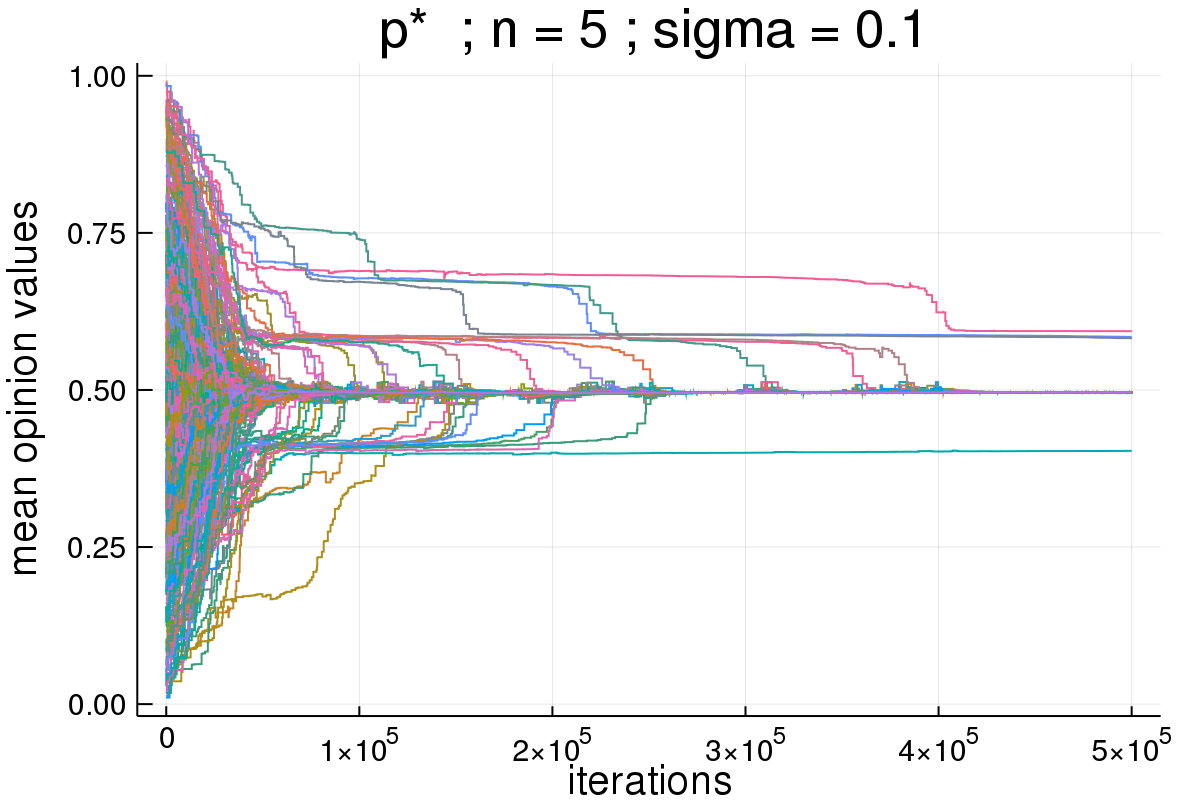
\includegraphics[width=\textwidth]{img/compare-ps/Poodlcalculatep*n5-rho10e-5-sigma01-00intrans.png}
        % \caption{\textcolor{red}{'ill fix thix}}
      \end{subfigure}
      \begin{subfigure}[b]{0.45\textwidth}
        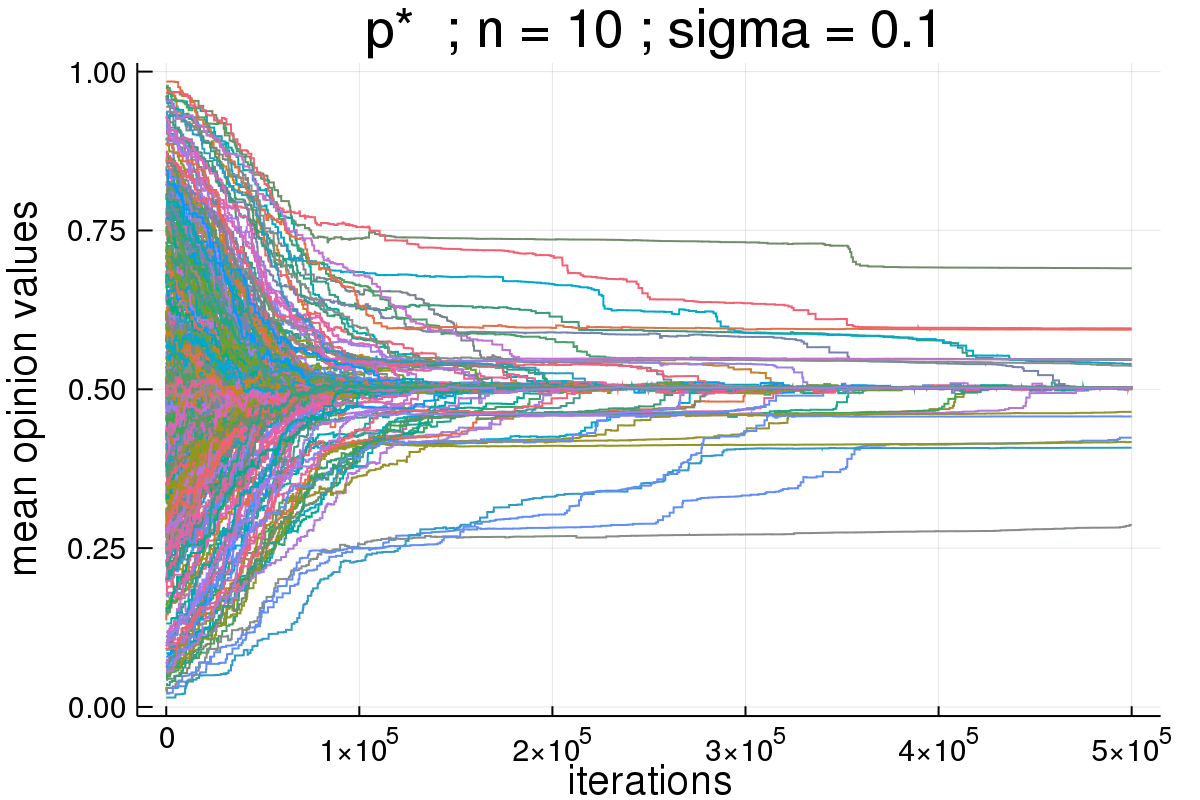
\includegraphics[width=\textwidth]{img/compare-ps/Poodlcalculatep*n10-rho10e-5-sigma01-00intrans.png}
        % \caption{\(n\_issues = 1, \sigma = 0.02\) }
      \end{subfigure}
      \begin{subfigure}[b]{0.5\textwidth}
        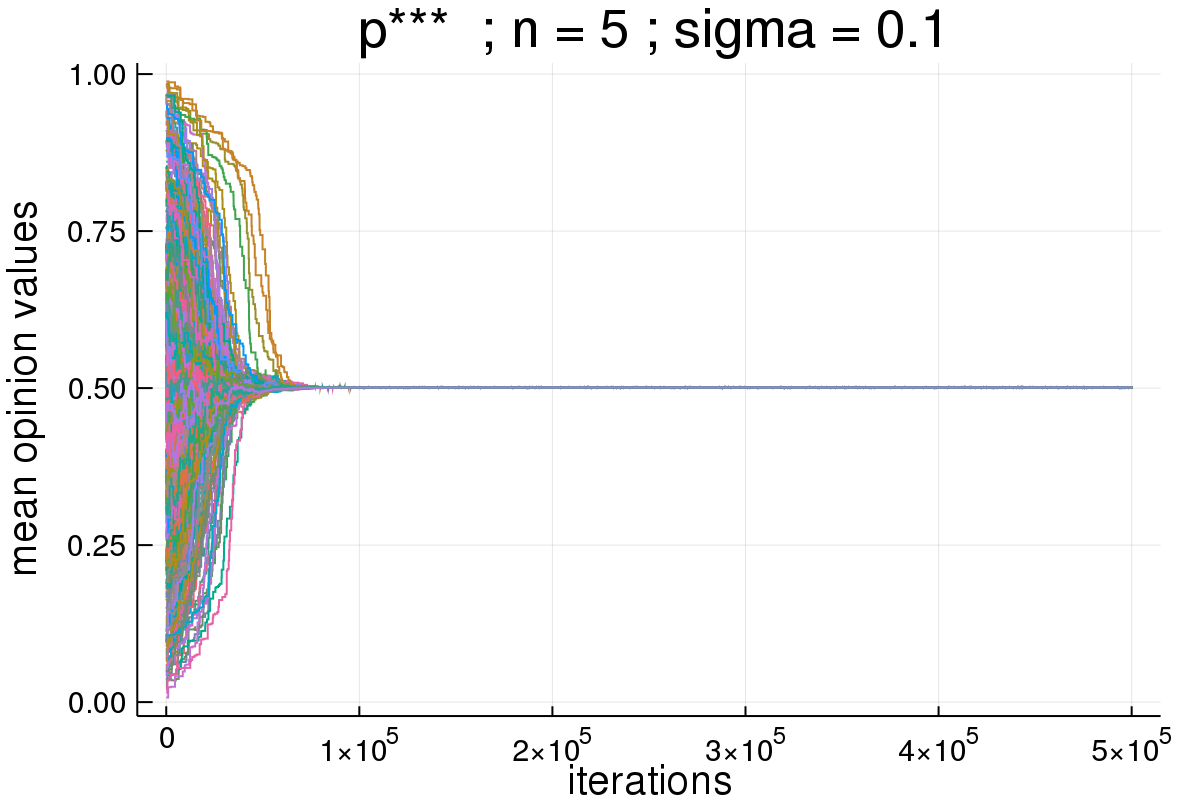
\includegraphics[width=\textwidth]{img/compare-ps/Poodlcalculatep***n5-rho1e-5-sigma01-00intrans.png}
        % \caption{\(n\_issues = 7, \sigma = 0.1\)}
      \end{subfigure}
  \label{fig:tseries4}
    \end{figure}

    

    
  \section{Conclusions}






\section{Acknowledgement}
The author would like to thank Funda\c{c}\~ao de Amparo \`a Pesquisa do Estado de S\~ao Paulo (FAPESP), for the support to this work, under grant %2008/00383-9.

\bibliographystyle{unsrt}
\bibliography{biblio}

\end{document}

%%% Local Variables:
%%% mode: latex
%%% TeX-master: t
%%% End:
